\documentclass[12pt, a4paper, UTF8, fontset=adobe, oneside]{ctexbook} % oneside 去掉所有空白页

\linespread{1.3} % 行距设置
\setcounter{secnumdepth}{3} % 层次为3以上的标题能够生成序号

%% 宏包
\usepackage{amsmath} % AMS数学宏包
\usepackage{fancyhdr} % 设置页眉页脚宏包
\usepackage{geometry} % 设置页边距宏包
\usepackage{xcolor} % 颜色宏包
\usepackage{hyperref} % 交叉引用宏包 colorlinks启用彩色模式 参考文献引用为紫红色
\usepackage[listings,breakable]{tcolorbox} % 彩色盒子宏包 代码宏包
\usepackage{enumitem} % 枚举设置宏包
\usepackage{tikz} % 画图宏包
\usepackage[europeanresistors]{circuitikz} % 电路绘制宏包
\usepackage[labelsep=quad]{caption} %标题宏包
% \usepackage{enumitem} %枚举环境宏包
\usepackage{graphicx} % 插图宏包
\usepackage{stmaryrd} % 平行符号

% 宏包设置
% 页眉页脚样式
\pagestyle{fancy} % 页面样式采用fancyhdr宏包中的fancy
\fancyhf{} % 去掉页眉
\cfoot{\thepage} % 页脚中间显示页码
\renewcommand{\headrulewidth}{0pt} % 去掉页眉的横线
% 页边距设置
\geometry{top = 2.54cm, bottom = 2.54cm, left = 3.18cm, right = 3.18cm}
% 章节样式设置
\CTEXsetup[name={第,部分},number={\arabic{part}}]{part}
\CTEXsetup[name={第,章},number={\arabic{chapter}}]{chapter}
% 插图目录
\graphicspath{{Figures/}}
% 文档设置
\renewcommand\contentsname{目录} % 中文 目录
\renewcommand\bibname{参考文献} % 中文 参考文献
% 清华紫
\definecolor{THU}{RGB}{111, 23, 135}
% 交叉引用宏包
\hypersetup{colorlinks=true,linkcolor=THU,citecolor=THU}
% tcolorbox样式设置
\newtcolorbox{redbox}[2][]{colback=yellow!10,colframe=red!75!black,coltitle=white,fonttitle=\bfseries,fontupper=\kaishu,title=#2,#1,center title,center upper,breakable} % 红色
\newtcolorbox{magbox}[2][]{colback=yellow!10,colframe=magenta!75!black,coltitle=white,fonttitle=\bfseries,fontupper=\kaishu,title=#2,#1,center title,center upper} % 紫红色
\newtcolorbox{THUbox}[2][]{colback=yellow!10,colframe=THU!75!black,coltitle=white,fonttitle=\bfseries,fontupper=\kaishu,title=#2,#1,center title,breakable} % 紫罗兰色
\newtcolorbox{THUCbox}[2][]{colback=yellow!10,colframe=THU!75!black,coltitle=white,fonttitle=\bfseries,fontupper=\kaishu,title=#2,#1,center title,center upper,breakable} % 紫罗兰色 居中
\newtcolorbox{purbox}[2][]{colback=yellow!10,colframe=purple!75!black,coltitle=white,fonttitle=\bfseries,fontupper=\kaishu,title=#2,#1,center title,center upper} % 紫色
\usetikzlibrary{calc,shapes.multipart,chains,arrows,positioning} % tikz library
\tikzset{circarrow/.style={*->,shorten <=-2pt}}

\begin{document}
\frontmatter
\begin{titlepage}
\begin{center}

\vspace*{5cm}
% Title
{\huge \bfseries 电力拖动自动控制系统理论}\\[0.4cm]

\vspace{12cm}

% {\large NCEPRI} \\[0.3cm]
{\large 江浩} \\[1cm]
{\large \today}

\end{center}
\end{titlepage}

\begin{titlepage}
\begin{center}

\end{center}
\end{titlepage}

{
\hypersetup{linkcolor=black} % 目录链接为黑色
\pagenumbering{Roman} % 页码编号为大写罗马数字
\tableofcontents % 目录
}

\mainmatter % 正文部分 重新编号
\pagenumbering{arabic} % 页码编号为阿拉伯数字

\part{交流调速系统}

\chapter{基于稳态模型的异步电动机调速系统}

\section{思考题}

\section{习题}
\subsection{第1题}
\subsubsection{题目}
一台三相笼型异步电动机的铭牌数据为:额定电压$U_{\mathrm{N}}=380\ \mathrm{V}$,额定转速$n_{\mathrm{N}}=960\ \mathrm{r/min}$,额定频率$f_{\mathrm{N}}=50\ \mathrm{Hz}$,定子绕组为Y联结。实验测得定子电阻$R_{\mathrm{s}}=0.35\ \Omega$,定子漏感$L_{\mathrm{ls}}=0.006\ \mathrm{H}$,定子绕组产生气隙主磁通的等效电感$L_{\mathrm{m}}=0.26\ \mathrm{H}$,转子电阻$R_r^{'}=0.5\ \Omega$,转子漏感$L_{r}^{'}=0.007\ \mathrm{H}$,转子参数已折合到定子侧,忽略铁心损耗。

(1) 画出异步电动机T形等效电路和简化等效电路。

(2) 求额定运行时的转差率$s_{\mathrm{N}}$,定子额定电流$I_{\mathrm{sN}}$和额定电磁转矩。

(3) 定子电压和频率均为额定值时,理想空载时的励磁电流$I_0$。

(4) 定子电压和频率均为额定值时,临界转差率$s_{\mathrm{m}}$和临界转矩$T_{\mathrm{m}}$,并画出该异步电机的机械特性。
\subsubsection{解答}
(1) 异步电机T形等效电路如图~\ref{Fig:TCircuit}所示。
\begin{figure}[htbp]
  \centering
  \begin{circuitikz}[scale=1.2]
    \draw 
    (0,0) node[anchor=east] {}
    to [short, o-] (4,0)
    (4.7,3) to [L=$L_m$, i>^=$\dot{I_0}$] (4.7,0)
    (0,3) node[anchor=west] {}
    to [short, o-] (0.2,3)
    to [R=$R_s$, i=$\dot{I_s}$] (2.5,3)
    to [L=$L_{ls}$] (4,3)
    to [L=$L_{lr}^{'}$, i<=$\dot{I_r^{'}}$] (8,3)
    (8,0) to [vR, l_=$\frac{R_r^{'}}{s}$] (8,3)
    (8,0) to [short, -] (4,0);
    \begin{scope}[>=stealth]
      \draw [->] (0.2,2.5) -- node[right]{$\dot{U_s}$} (0.2,0.5);
    \end{scope}
  \end{circuitikz}
  \caption{异步电机T形等效电路图}\label{Fig:TCircuit}
\end{figure}

(2)额定运行时的转差率为
\begin{equation}
  s_{\mathrm{N}}=\dfrac{1000-960}{1000}=0.04
\end{equation}

定子额定电流为
\begin{equation}
  \left| I_{\mathrm{s}} \right| = \left| {\dfrac{U_{\mathrm{s}}}{R_{\mathrm{s}}+\mathrm{j}\omega_1L_{\mathrm{ls}}+\mathrm{j}\omega_1L_{\mathrm{m}} \sslash (R_{\mathrm{r}}^{'}+\mathrm{j}\omega_1L_{\mathrm{lr}})}} \right| = 28.66\ \mathrm{A}
\end{equation}

额定电磁转矩为(忽略励磁电流)
\begin{equation}
  T_{\mathrm{e}} = \dfrac{3pU_{\mathrm{s}}^2R_{\mathrm{r}}^{'}s}{\omega_1[(sR_{\mathrm{s}}+R_{\mathrm{r}}^{'})^2+s^2\omega_1^2(L_{\mathrm{ls}}+L_{\mathrm{lr}})^2]} = 272.84\ (\mathrm{N·m})
\end{equation}

(3)理想空载时的励磁电流为
\begin{equation}
  \left| I_0 \right| = \left| \dfrac{U_{\mathrm{s}}}{R_{\mathrm{s}}+\mathrm{j}\omega_1L_{\mathrm{ls}}+\mathrm{j}\omega_1L_{\mathrm{m}}} \right| = 4.48\ \mathrm{A}
\end{equation}

(4)临界转差率为
\begin{equation}
  s_{\mathrm{m}} = \frac{R_{\mathrm{r}}^{'}}{\sqrt{R_{\mathrm{s}}^2+\omega_1^2(L_{\mathrm{ls}}+L_{\mathrm{lr}}^{'})^2}}=0.1220
\end{equation}

临界转矩为
\begin{equation}
  T_{\mathrm{em}}=\dfrac{3pU_{\mathrm{s}}^2}{2\omega_1(R_{\mathrm{s}}+\sqrt{R_{\mathrm{s}}^2+\omega_1^2(L_{\mathrm{ls}}+L_{\mathrm{lr}})^2})} = 464.90\ (\mathrm{N·m})
\end{equation}

机械特性曲线如图~\ref{Fig:MechCurve}所示。

\begin{figure}[htbp]
  \centering
  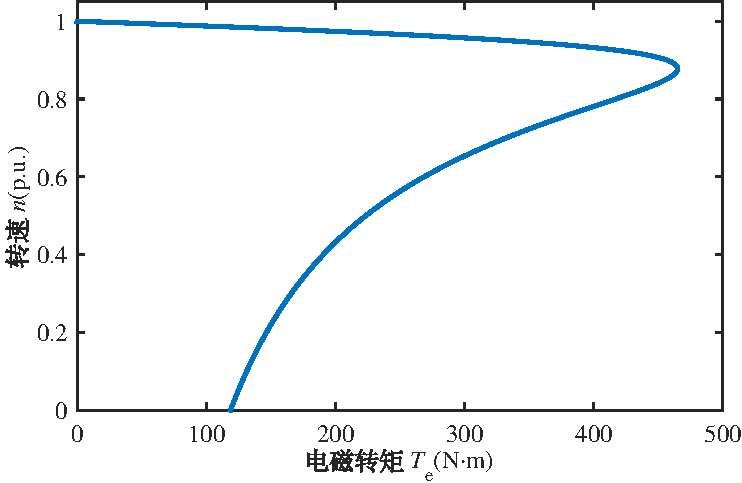
\includegraphics[width=12.557cm]{Fig_T_s.pdf} % 设置宽度保持字号不变
  \caption{异步电机的机械特性}\label{Fig:MechCurve}
\end{figure}

\subsection{第2题}
\subsubsection{题目}
异步电动机参数如第1题所示,画出调压调速在$\dfrac{1}{2}U_{\mathrm{N}}$和$\dfrac{2}{3}U_{\mathrm{N}}$时的机械特性,计算临界转差率$s_{\mathrm{m}}$和临界转矩$T_{\mathrm{m}}$,分析气隙磁通的变化。分析在恒转矩负载情况下,调压调速的稳定运行范围。
\subsubsection{解答}
由于临界转差率$s_{\mathrm{m}} = \frac{R_{\mathrm{r}}^{'}}{\sqrt{R_{\mathrm{s}}^2+\omega_1^2(L_{\mathrm{ls}}+L_{\mathrm{lr}}^{'})^2}}$,因此在不同电压下,临界转差率不变。

临界电磁转矩为
\begin{align}
  T_{\mathrm{m}}(U=\frac{1}{2}U_{\mathrm{N}}) = 116.22 (\mathrm{N·m}) \\
  T_{\mathrm{m}}(U=\frac{2}{3}U_{\mathrm{N}}) = 206.62 (\mathrm{N·m})
\end{align}

气隙磁通公式为
\begin{equation}
  \Phi_{\mathrm{m}}\approx\frac{U_{\mathrm{s}}}{4.44f_1N_{\mathrm{s}}k_{\mathrm{N}_{\mathrm{s}}}}
\end{equation}

因此,电压下降将导致气隙磁通减小。

对恒转矩负载而言,调速范围为额定电压下稳态运行时的转差率对应的转速与临界转差率对应的转速之间。

\subsection{第3题}
\subsubsection{题目}
异步电动机参数如第1题所示,定子每相绕组匝数$N_{\mathrm{s}}=125$,定子基波绕组系数$k_{\mathrm{N}_{\mathrm{s}}}=0.92$,定子电压和频率均为额定值。

(1) 忽略定子漏阻抗,每极气隙磁通量$\Phi_{\mathrm{m}}$和气隙磁通在定子每相中感应电动势的有效值$E_{\mathrm{g}}$。

(2) 考虑定子漏阻抗,求理想空载和额定负载时的$\Phi_{\mathrm{m}}$和$E_{\mathrm{g}}$。

(3) 比较上述三种情况下,$\Phi_{\mathrm{m}}$和$E_{\mathrm{g}}$的差异,并说明原因。
\subsubsection{解答}
(1) 忽略定子漏阻抗,则有 $E_{\mathrm{g}} = U_{\mathrm{s}} = 380\ \mathrm{V}$,每极气隙磁通量为

\begin{equation}
  \Phi_{\mathrm{m}} = \frac{E_{\mathrm{g}}}{4.44f_1N_{\mathrm{s}}k_{\mathrm{N}_{\mathrm{s}}}} = 0.0149\ \mathrm{(Wb)}
\end{equation}

(2) 考虑定子漏阻抗时,理想空载情况下,定子每相感应电动势为
\begin{equation}
  \left| E_{\mathrm{g}} \right|=\left| \dfrac{\mathrm{j}X_{\mathrm{m}}}{R_{\mathrm{s}}+\mathrm{j}X_{\mathrm{s}}+\mathrm{j}X_{\mathrm{m}}} U_{\mathrm{s}} \right| = 371.42\ (\mathrm{V})  
\end{equation}

每极气隙磁通量为
\begin{equation}
  \Phi_{\mathrm{m}} = \frac{\left|E_{\mathrm{g}}\right|}{4.44f_1N_{\mathrm{s}}k_{\mathrm{N}_{\mathrm{s}}}} = 0.0145\ \mathrm{(Wb)}
\end{equation}

额定负载情况下,定子每相感应电动势为
\begin{equation}
  \left| E_{\mathrm{g}} \right| = \left|{\dfrac{\mathrm{j}\omega_1L_{\mathrm{m}} \sslash (R_{\mathrm{r}}^{'}+\mathrm{j}\omega_1L_{\mathrm{lr}})U_{\mathrm{s}}}{R_{\mathrm{s}}+\mathrm{j}\omega_1L_{\mathrm{ls}}+\mathrm{j}\omega_1L_{\mathrm{m}} \sslash (R_{\mathrm{r}}^{'}+\mathrm{j}\omega_1L_{\mathrm{lr}})}} \right| = 350.33\ \mathrm{V}
\end{equation}

\begin{equation}
  \Phi_{\mathrm{m}} = \frac{\left|E_{\mathrm{g}}\right|}{4.44f_1N_{\mathrm{s}}k_{\mathrm{N}_{\mathrm{s}}}} = 0.0137\ \mathrm{(Wb)}
\end{equation}


\subsection{第4题}
\subsubsection{题目}
接上题,求:

(1) 

(2)

(3)
\subsubsection{答案}

\bibliographystyle{thubib}
\bibliography{refs}
\end{document}

%%% Local Variables:

\bibliographystyle{thubib}
\bibliography{refs}
\end{document}

%%% Local Variables:
%%% TeX-master: t
%%% End:
